\documentclass[crop,tikz]{standalone}% 'crop' is the default for v1.0, before it was 'preview'
%\usetikzlibrary{...}% tikz package already loaded by 'tikz' option

\usetikzlibrary{arrows,positioning} 
\usetikzlibrary{shapes,decorations}
\usetikzlibrary{calc}
\usetikzlibrary{fit}
\usetikzlibrary{decorations.pathreplacing}
\usetikzlibrary{backgrounds}


\renewcommand{\familydefault}{\sfdefault}


\definecolor{blind_red}{HTML}{D7191C}
\definecolor{blind_orange}{HTML}{FDAE61}
\definecolor{blind_yellow}{HTML}{FFFFBF}
\definecolor{blind_blue}{HTML}{ABD9E9}
\definecolor{blind_blue2}{HTML}{2C7BB6}



\begin{document}
	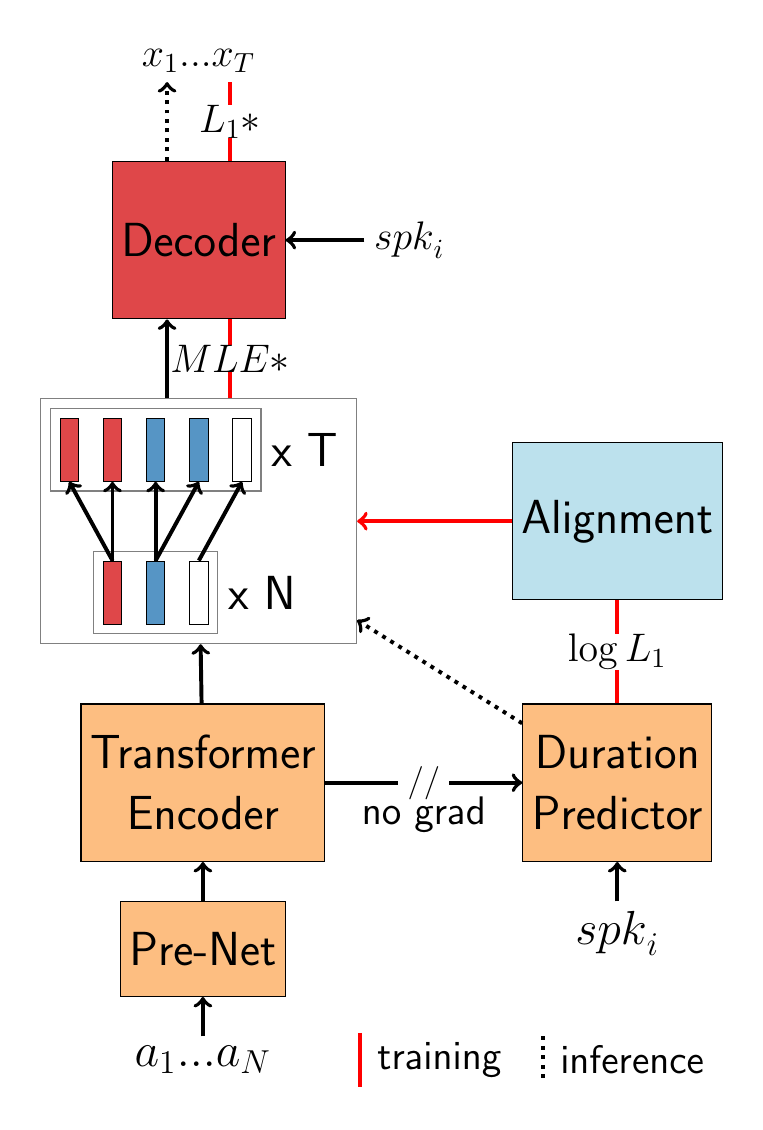
\begin{tikzpicture}[
	    auto,
	    background rectangle/.style={fill=white}, show background rectangle,
	    onlytext/.style={align=center, font=\LARGE},
        halfbox/.style={rectangle, minimum size=1.20cm, draw, font=\LARGE},
	    box/.style={rectangle, minimum size=2.00cm, draw, font=\LARGE},
	    halforangebox/.style={halfbox, fill=blind_orange!80},
	    orangebox/.style={box, fill=blind_orange!80},
	    normalline/.style={->, line width=0.5mm},
	    state/.style={rectangle, draw, minimum height=0.8cm, minimum width=0.2cm},
	]
	% Encoder
    \node[halforangebox, align=center] (prenet) at (0, 0) {Pre-Net};
    \node[onlytext, below=0.5cm of prenet] (inlabel) {$a_1 ... a_N$};
    \node[orangebox, align=center, above=0.5cm of prenet] (encoder) {Transformer\\Encoder};
    \node[orangebox, align=center, right=2.5cm of encoder] (dp) {Duration\\Predictor};
    \node[onlytext, below=0.5cm of dp] (dpspk) {${spk}_i$};

    %Upsamling stuff
    \def \statesep {0.3cm}

    \node[state, above=1cm of encoder, fill=blind_blue2!80, xshift=-0.6cm] (estate2) {};
    \node[state, left=\statesep of estate2, fill=blind_red!80] (estate1) {};
    \node[state, right=\statesep of estate2] (estate3) {};

    \node [draw=black!50, fit={(estate1) (estate2) (estate3)}] (estatebox) {};

    \node [onlytext, right=0.0cm of estatebox] (estatelabel) {x N};

    \node[state, above=1cm of estate2, fill=blind_blue2!80] (dstate3) {};
    \node[state, left=\statesep of dstate3, fill=blind_red!80] (dstate2) {};
    \node[state, left=\statesep of dstate2, fill=blind_red!80] (dstate1) {};
    \node[state, right=\statesep of dstate3, fill=blind_blue2!80] (dstate4) {};
    \node[state, right=\statesep of dstate4] (dstate5) {};

    \node [draw=black!50, fit={(dstate1) (dstate2) (dstate3) (dstate4) (dstate5)}] (dstatebox) {};

    \draw [normalline] (estate1.north) -- (dstate1.south);
    \draw [normalline] (estate1.north) -- (dstate2.south);

    \draw [normalline] (estate2.north) -- (dstate3.south);
    \draw [normalline] (estate2.north) -- (dstate4.south);

    \draw [normalline] (estate3.north) -- (dstate5.south);

    \node [onlytext, right=0.0cm of dstatebox] (dstatelabel) {x T};

    \coordinate (aligncenter) at ($(estate1.north)!.5!(dstate3.south)$);

    \node [draw=black!50, fit={(estatebox) (dstatebox) (dstatelabel)}] (upsamplebox) {};

    \path let \p1 = (dp), \p2 = (aligncenter) in node at (\x1, \y2) [box, align=center, fill=blind_blue!80] (alignment)  {Alignment};

    % Decoder
    \node[box,fill=blind_red!80, align=center, above=1.0cm of upsamplebox] (decoder) {Decoder};
    \node[right=1cm of decoder] (decspk) {\Large ${spk}_i$};
    \node[above=1.0cm of decoder] (logmel) {\Large $x_1 ... x_T$};

    % connection lines
    \draw [normalline] (inlabel) -- (prenet);
    \draw [normalline] (prenet) -- (encoder);
    \draw [normalline] (dpspk) -- (dp);
    \draw [normalline] (encoder) -- ++(dp) node [anchor=center, midway, fill=white] (gradstop) {\large //};
    \node [below=-0.3cm of gradstop] (nogradlabel) {\Large no grad};
    \draw [normalline] (encoder) -- (upsamplebox);
    \draw [normalline, red] (alignment) -- (upsamplebox);
    \draw [normalline] ([xshift=-0.4cm]upsamplebox.north) -- ([xshift=-0.4cm]decoder.south);
    \draw [normalline] (decspk) -- (decoder);
    \draw [normalline, dotted] (dp) -- (upsamplebox);

    % Losses
    \draw [line width=0.5mm, red] (dp) -- (alignment) node [black, anchor=center, midway, fill=white, inner sep=0] {\Large $\log L_1$};
    \draw [line width=0.5mm, red] ([xshift=0.4cm]upsamplebox.north) -- ([xshift=0.4cm]decoder.south) node [black, anchor=center, midway, fill=white, inner sep=0] (mfeloss) {\Large $MLE*$};
    \draw [line width=0.5mm, red] ([xshift=0.4cm]logmel.south) -- ([xshift=0.4cm]decoder.north) node [black, anchor=center, midway, fill=white, inner sep=0] (l1loss) {\Large $L_1*$};
    \draw [normalline, dotted] ([xshift=-0.4cm]decoder.north) -- ([xshift=-0.4cm]logmel.south);

		% Legend
		\node[right=0.6cm of inlabel, xshift=0.5cm] (trainingline) {\Large training};
		\draw [line width=0.5mm, red] ([xshift=-0.1cm]trainingline.north west) -- ([xshift=-0.1cm]trainingline.south west);

		\node[right=0.5cm of trainingline] (inferenceline) {\Large inference};
		\draw [line width=0.5mm, dotted] ([xshift=-0.1cm]inferenceline.north west) -- ([xshift=-0.1cm]inferenceline.south west);

	\end{tikzpicture}
\end{document}